\begin{document}
	\chapter{Implementation}
	This chapter describes how the requirements highlighted previously have been accomplished. 
	\section{Overall structure of the project} \label{Section: impl/overview}
	The main objective I had while implementing the project was to be able to have an independent tool that can communicate with the CADETS client and classify nodes successfully. In order to achieve this, I divided the overall project into three smaller sub-modules:
	\begin{enumerate}
		\item \label{impl/overview/enum/1} The \textbf{Neo4J interface}, which handles the interaction between my tool and the Neo4J database that stores the graph data with the end purpose of extracting the nodes' feature vectors (Section \ref{Section: impl/neo4j}).
		
		\item The \textbf{machine learning module}, which uses the feature vectors extracted by the \ref{impl/overview/enum/1}$^{\text{st}}$ module in order to classify the nodes into \textit{SHOW} or \textit{HIDE} (Section \ref{Section: impl/ml}).
		
		\item The \textbf{REST API}, which wraps around the previous two modules and handles requests received by the tool (Section \ref{Section: impl/REST}).
	\end{enumerate}
	Figure \ref{Fig: impl/pipeline} shows a schema of how the 3 modules will work together as a part of a request processing pipeline. 
	\\ \\
	In the following sections, I will give a detailed description of theses modules in a bottom-up approach -- from the Neo4J interaction to the REST API. 
	\begin{figure}[H]
		\centering
		\includegraphics[width=.95\textwidth]{graphics/overall-schema}	
		\caption[Processing pipeline]{Overview of the project's processing pipeline.}
		\label{Fig: impl/pipeline}
	\end{figure}
	\section{Neo4J interaction} \label{Section: impl/neo4j}
	This section describes the implementation of the Neo4J interaction module and how the nodes' features are extracted. 
	\subsection{Database driver} \label{Section: impl/neo4j/driver}
	The biggest challenge when designing the database driver was the choice of the library I would use to run the actual queries. There are a number of Python libraries available, out of which I took two into consideration: \textbf{py2neo}\footnote{\textbf{\url{http://py2neo.org/v3/}}} and \textbf{neo4j-driver}\footnote{\textbf{\url{https://github.com/neo4j/neo4j-python-driver}}}. In order to decide which one I would use, I timed both libraries while running two queries and the overall feature extraction for one node on a database of $631, 357 \text{ nodes}$. The resulting times are shown in Table \ref{Table: impl/neo4j-driver-timings}:
	\begin{longtable}{|p{.15\textwidth}|p{.30\textwidth}p{.25\textwidth}p{.25\textwidth}|}
		\textbf{library} & \textbf{\textit{match(n) return n}} & \textbf{\textit{match(n) return n limit 1}} & \textbf{feature extraction} \\
		\hline
		\textit{py2neo} & $337.477\text{s } (\approx5.5 \text{ minutes})$ & $13\text{ms}$ & $85.15\text{s}$ \\ 
		\textit{neo4j-driver} & $97.288\text{s }(\approx1.5 \text{ minutes})$ & $28\text{ms}$ & $68.78\text{s}$  \\
		\hline
		\caption[Neo4J libraries timings]{\centering Timings for the two Neo4J libraries considered.}
		\label{Table: impl/neo4j-driver-timings}
	\end{longtable}
	The main purpose of the database driver is to support feature extraction. Therefore, given the times in Table \ref{Table: impl/neo4j-driver-timings}, I decided to use \textbf{neo4j-driver}. On top of this library, I wrote a wrapper class, \textbf{DatabaseDriver}. 
	\subsection{Feature extractor} \label{Section: impl/neo4j/features}
	The feature extractor uses the DatabaseDriver class described previously in order to build the feature vectors for a list of nodes, just as described in Table \ref{Table: prep/features}. The UML diagram from Figure \ref{Fig: impl/neo4j-driver-uml} illustrates the relationships between the two classes.
	\\ \\
	In order to ensure that the models are well-behaved, I decided to use \textbf{one-hot-encoding} for the categorical features. In other words, for every such feature, I generated an extra boolean column for each category. Only one of these columns can take the value 1 for each sample. Using this encoding led to an increase in the length of the feature vectors, from 13 to 23 variables. 
	\begin{figure}[H]
		\centering
		\includegraphics[width=.5\textwidth]{graphics/umls/uml-neo4j-driver}
		\caption[FeatureExtractor UML class diagram]{\centering UML class diagram showing the FeatureExtractor and the DatabaseDriver classes.}
		\label{Fig: impl/neo4j-driver-uml}
	\end{figure}
	\section{Machine learning module} \label{Section: impl/ml}
	With the first module being implemented, I started to look into different machine learning models that I would use to classify the nodes. 
	\subsection{Training set} \label{Section: impl/ml/training-set}
	One of the key requirements for a well-behaved machine learning model is to have a comprehensive training set. Keeping this in mind, I used the ground-truths listed in Section \ref{Section: prep/data/ground-truths} with the aim of extracting examples of nodes from both classes (i.e. \textit{SHOW} and \textit{HIDE}) from a database of $6,008$ nodes, out of which $5,498$ are of interest (i.e. either \textit{File}, \textit{Process} or \textit{Socket}). For all these nodes, I used the feature extractor in order to build a labelled training set $\mathbf{s}=\{ (\mathbf{x}_1, \mathbf{y_1}), \dots, (\mathbf{x}_n, \mathbf{y_n}) \}$ that will be used by all the models in the training phase. As expected, there is an imbalance in the training data, with $2,382$ nodes ($43.33\%$) labelled as \textit{SHOW} and $3,115$ ($56.67\%$) labelled as \textit{HIDE}. This is a factor that I took into consideration when designing the models.
	
	\subsection{The Keras environment} \label{Section: impl/ml/ecosys}
	Keras is a high-level deep-learning API, that can run on top of TensorFlow\footnote{\textbf{\url{https://www.tensorflow.org/}}}, CNTK\footnote{\textbf{\url{https://github.com/Microsoft/cntk}}} or Theano\footnote{\textbf{\url{https://github.com/Theano/Theano}}}, providing user friendliness, modularity and extensibility. It allows for easy and fast prototyping, fitting well with the software engineering approach I took during the implementation stage. Moreover, Keras modules are highly portable: a model developed using one backend can just as easily work on any other accepted backend. For the implementation of the parametric techniques I experimented with as part of this project, I used the TensorFlow backend for Keras. 
	\\ \\
	The core data structure of Keras is a \textbf{Model}, an abstraction that gives users the ability to organize different types of layers. For the models presented here, I used the \textbf{Sequential} model, which represents a linear stack of layers. Running a model in Keras consists of 4 core actions:
	\begin{enumerate}
		\item \textbf{definition} - initialising the model and using the \textit{.add()} method to add layers.
		
		\item \textbf{compilation} - using the \textit{.compile()} method to define the loss function and optimizer used during the training phase, as well as any hyperparameters that they require. At this stage, one can also define the metrics used in evaluation. 
		
		\item \textbf{training} - once the model was compiled, the \textit{.train()} is be used to define the training and validation sets used for optimizing the weights and hyperparameters of the model, respectively. Here, the user can define two other hyperparameters: the number of iterations for which the optimizer will run and the batch size)( for batch-based optimisation methods). 
		
		\item \textbf{running} - with the model being optimized, the user can either use it to make predictions or to evaluate it, using the metrics defined in the compile stage. 
	\end{enumerate}
	The \textit{ModelCheckpoint} callback was used to save the pre-trained parameters of a given model to disk. These checkpoints can then be loaded using the \textit{load\_weights()} method. Therefore, my implementation does not require training the model every time the application starts and is time efficient.
	
	\subsection{Overview} \label{Section: impl/ml/overview}
	In order to choose the most suitable model for the data I am working on, I first implemented a number of different machine learning algorithms and then comparatively evaluated them. This way, I could understand each model's suitability and performance on this fine-grained provenance data. One of the key properties I was looking for was the robustness to the imbalance in the labels assigned to nodes. The models implemented and reasoning behind them are outlined in Table \ref{Table: impl/ml/overview/models} and detailed in the following sections.
	\\ \\
	\begin{longtable}{|p{.30\textwidth}|p{.60\textwidth}|}
		\textbf{Model} & \textbf{Implementation reason} \\
		\hline
		\textit{Logistic Regression} & Is the simplest classification algorithm and therefore I used it as a baseline for the other models to be compared against. \\
		\hline 
		\textit{Multilayer Perceptron} & Adds a number of nonlinearities compared to logistic regression and therefore should identify relationships between features better. Yet, being simple and lightweight, should result in faster training and classification. \\
		\hline
		\textit{Convolutional Neural Network} & When using dilated convolution on an input vector, we can identify more relationships between the features than the previous models. \\
		\hline
		\textit{Probabilistic Neural Network} & I wanted to experiment with a non-parametric technique, such as PNNs, which, given sufficient data, should overcome some of the limitations of the other models. \\
		\hline
		\caption{Models implemented as part of this project.}
		\label{Table: impl/ml/overview/models}
	\end{longtable}

	Throughout the implementation stage, I carefully followed the object-oriented paradigm, making use of class inheritance. For this reason, when implementing the machine learning models I first declared an abstract base class, \textit{Model} (Figure \ref{Fig: impl/ml/model/uml/model}). The \textit{model} variable is an instance of Keras' \textit{Sequential} class, used to actually run the model. I made this choice keeping in mind that some models (such as the PNN described in Section \ref{Section: impl/ml/pnn}) do not make use of the Keras API. 
	\\ \\
	The \textit{config} variable is used to determine whether the model is being trained, evaluated or simply used for predicting the corresponding classes.
	\begin{figure}[H]
		\centering
		\begin{subfigure}[b]{.3\textwidth}
			\includegraphics[width=\textwidth]{graphics/umls/model-uml}
			\caption{The \textit{Model} class}
			\label{Fig: impl/ml/model/uml/model}
			\hspace{1pt}
		\end{subfigure}\hfill
		\begin{subfigure}[b]{.55\textwidth}
			\includegraphics[width=\textwidth]{graphics/umls/model-cnf-uml}
			\caption{The types of configurations used}
			\label{Fig: impl/ml/model/uml/configs}
		\end{subfigure}
		\caption{\textit{Left:} UML of the \textit{Model} abstract class. \textit{Right:} Different types of configurations used.}
		\label{Fig: impl/ml/model/uml}
	\end{figure}
	The three core methods of the $Model$ class will be implemented in classes inheriting from it. Table \ref{Table: impl/ml/model/purpose} explains how each method should be implemented by these classes.
	\begin{longtable}{p{.3\textwidth}p{.6\textwidth}}
		\textbf{method} & \textbf{purpose} \\
		\hline
		\textit{setup()} & Defining the elements of the model and, if in the \textit{models.config.PredictConfig} mode, loading the optimised parameters from disk. \\
		\hline
		\textit{train()} & Optimising the parameters of the model and saving the checkpoint on disk. Only accessible in \textit{models.config.TrainConfig} and \textit{models.config.EvalConfig} modes. \\
		\hline
		\textit{predict()} & Given a feature matrix, runs the model and returns the resulting probability distributions. Only accessible in the \textit{models.config.PredictConfig} mode.\\
		\hline
		\caption{Abstract methods of the \textit{Model} class explained}
		\label{Table: impl/ml/model/purpose}
	\end{longtable}

	\subsection{Regularization techniques} \label{Section: impl/ml/reg}
	When training neural networks, one of the most frequent problems is \textbf{overfitting}: the model corresponds too closely to the training data and therefore fails to generalize as expected. This section addresses the techniques applied in order to avoid this issue.
	\subsubsection{Batch normalization} \label{Section: impl/ml/reg/batch}
	During the training phase, the distribution of each layer's input changes, as the parameters of the previous layer change, phenomenon known as \textit{internal covariance}. This slows down the training by requiring lower learning rates and careful parameter initialisation. 
	\\ \\
	In this section, I describe \textbf{batch normalization}\cite{DBLP:journals/corr/IoffeS15}, a technique which addresses this problem, by normalizing the layer inputs for every training mini-batch. 
	\\ \\
	Let $\{ \mathbf{x}_1, \dots, \mathbf{x}_m  \}$ be the input elements for a layer in the network. Each scalar feature is normalized independently, by making it have mean $\mu = 0$ and variance $\sigma = 1$.  The normalized input $\mathbf{\hat{x}}_k$ is computed as follows:
	\begin{equation}
		\mathbf{\hat{x}}_k = \frac{\mathbf{x}_k - \mu}{\sqrt{\sigma + \epsilon}}
	\end{equation}
	where $\epsilon > 0$ is a constant used to avoid division by zero and $\mu$ and $\sigma$ are the mean and variance of the original vector $\mathbf{x}_k$. Namely:
	\begin{longtable}{ccc}

				$\mu = \frac{1}{m} \sum_{1}^{m} x_i$

			&   and   &

				$\sigma = \sqrt{\frac{1}{m}\sum_{1}^{m}(x_i - \mu)}$

	\end{longtable}
	By learning a scale ($\gamma$) and a shift ($\beta$) parameter, the model can fall back to the original values. The final output of BatchNorm is: 
	\begin{equation}
		\mathbf{z}_k = \gamma \mathbf{\hat{x}}_k + \beta
	\end{equation} 
	\subsubsection{Dropout} \label{Section: impl/ml/reg/dropout}
	Dropout\cite{dropout} is a regularization technique applied during training to reduce overfitting in neural networks. The term 'dropout' refers to  dropping out units (both hidden and visible) - temporarily removing them from the neural network, along with all of their incoming and outgoing connections, as shown in Figure \ref{Fig: impl/ml/dropout}. The choice of which units are dropped is random.
	\begin{figure}[H]
		\centering
		\includegraphics[width=.8\textwidth]{graphics/nns/dropout}
		\caption{\textit{Left:} MLP without using dropout. \textit{Right:} MLP after dropout is applied. The red crosses signify the neurons removed during training.}
		\label{Fig: impl/ml/dropout}
	\end{figure}
	Each unit is retained with a fixed \textbf{keep probability} $k_p$, independently of other units in the network. Since dropout is only applied during training, the weights corresponding to a unit need to be scaled by $\frac{1}{k_p}$ at test time.
	
	\subsection{Baseline model} \label{Section: impl/ml/baseline}
	As a baseline I implemented \textbf{logistic regression}, a single-neuron model that uses softmax as its activation function in order to generate the probability distributions over the two classes: \textit{SHOW} and \textit{HIDE}. The node represented by the feature vector $\textbf{x}$ is then assigned the class with the maximum probability $\mathbb{P}(C_i\mid \mathbf{x})$:
	\begin{equation}
	\centering
	\begin{split}
		C & = \argmax_{C_i} \mathbb{P}|(C_i\mid \mathbf{x}) \\
		  & = \argmax_{C_i} (\text{softmax}_i (\mathbf{w}^T\mathbf{x}))
	\end{split}
	\end{equation} 
	The optimizer used in this case was \textbf{mini-batch gradient descent}, with learning rate $\lambda = 0.01$. The loss function used was \textbf{binary crossentropy}, a special case of categorical crossentropy that applies to 2-class classification problems, such as the one I am trying to solve. 
	
	\subsection{Multilayer perceptron} \label{Section: impl/m/mlp}
	This section describes the implementation of the second model used as part of this project: the multilayer perceptron (MLP). In practice, an MLP architecture consists of an \textit{expansion phase}, where the number of neurons in the hidden layers increases and a \textit{reduction phase}, where their number decreases. This way, the features in the input data are combined in the expansion phase, while the most important features are selected in the reduction phase, in order to determine the class.
	\\ \\
	The MLP architecture I found most appropriate for the data used in my project consists of 4 layers, as shown in Figure \ref{Fig: impl/ml/mlp}. The first layer is the input layer, consisting of 23 neurons (the  length of each feature vector). It is followed by two hidden layers: one with 32 neurons (the expansion phase) and one consisting of 16 neurons (the reduction phase). The output layer has two neurons, representing $\mathbb{P}(C|\mathbf{x})$ - the probability that a feature vector $\mathbf{x}$ belongs to a class $C \in \{ SHOW, HIDE \}$.
	\begin{figure}[H]
		\centering
		\includegraphics[width=.9\textwidth]{graphics/nns/mlp-impl}
		\caption{MLP architecture}
		\label{Fig: impl/ml/mlp}
	\end{figure} 

	The ReLU activation function was chosen for the first three layers of the MLP due to its linear non-saturating form. Moreover, research has shown that it significantly accelerates the convergence of the optimisation algorithm\cite{Nair:2010:RLU:3104322.3104425}. The output layer uses the softmax activation function in order to get the probability distribution over the two classes. 
	\\ \\
	The input and hidden layers use batch normalization in order to avoid overfitting. For the same reason, I also applied dropout to these layers, with a keep probability $k_p = 0.8$. Figure \ref{Fig: impl/ml/mlp/compgraph} shows the computational graphs for the input and hidden layers (\ref{Fig: impl/ml/mlp/compgraph-hidden}) and the output layer (\ref{Fig: impl/ml/mlp/compgraph-output}), respectively.
	\subsubsection*{Training the MLP}
	The loss function used for this model computes the binary crossentropy between the output distribution and the one-hot encoded labels from the trainig set. On top of this, I am using weight decay as a regularization technique in order to control the model's complexity by penalizing large weights. The final loss function has the following form:
	\begin{equation}
		\mathfrak{L} = - y_{C_1}\log(y'_{C_1}) - y_{C_2}\log(y'_{C_2}) + \frac{\alpha}{2}\vert\vert\mathbf{w}\vert\vert 
		\label{Eq: impl/ml/loss}
	\end{equation}
	where $C_1$ and $C_2$ are the \textit{SHOW} and \textit{HIDE} classes, $\alpha$ is a hyperparameter and $\vert\vert\mathbf{w}\vert\vert$ is the $L_2$ norm of the weight vector ($\vert\vert\mathbf{w}\vert\vert = \sqrt{\sum \vert w_i^2 \vert}$).
	\\ \\
	Adam\cite{DBLP:journals/corr/KingmaB14}, a variation of mini-batch gradient descent, is the algorithm used to optimize the model. Adam is more computationally effective than other optimization algorithms, requiring just the first-order gradients to be computed and having lower memory requirements. It computes individual adaptive learning rates for different parameters from the first and second moments of the gradients. A more detailed explanation of how it works can be found in Appendix \ref{appendix-MLP-opt}, Section \ref{Appendix: Adam}.

	\begin{figure}[H]
		\centering
		\begin{subfigure}[b]{.4\textwidth}
			\includegraphics[width=\textwidth]{graphics/nns/mlp-compGraph}
			\caption{Input \& hidden layer}
			\label{Fig: impl/ml/mlp/compgraph-hidden}
		\end{subfigure}
		\hfill
		\begin{subfigure}[b]{.4\textwidth}
			\includegraphics[width=\textwidth]{graphics/nns/ml-compGraphOutput}
			\caption{Output layer}
			\label{Fig: impl/ml/mlp/compgraph-output}
	\end{subfigure}
	\caption[Computational graphs for MLP layers]{\textit{Left:} The computational graph for an input/ hidden layer. \textit{Right:} The computational graph for the output layer.}
	\label{Fig: impl/ml/mlp/compgraph}
	\end{figure}
	
	\subsection{Convolutional Neural Network} \label{Section: impl/ml/cnn}
	In this section I describe the implementation of the Dilated Convolutional Neural Network. From an architectural point of view, the CNN consists of: 1 input layer, with 23 neurons, 3 single-dimensional dilated convolutional layers that increase the size of the feature vector from $1\times23$ to $1\times128$, 1 fully connected hidden layer and 1 output layer. Figure \ref{Fig: impl/ml/cnn/architecture} shows the architecture schema. 
	\begin{figure}[H]
		\centering
		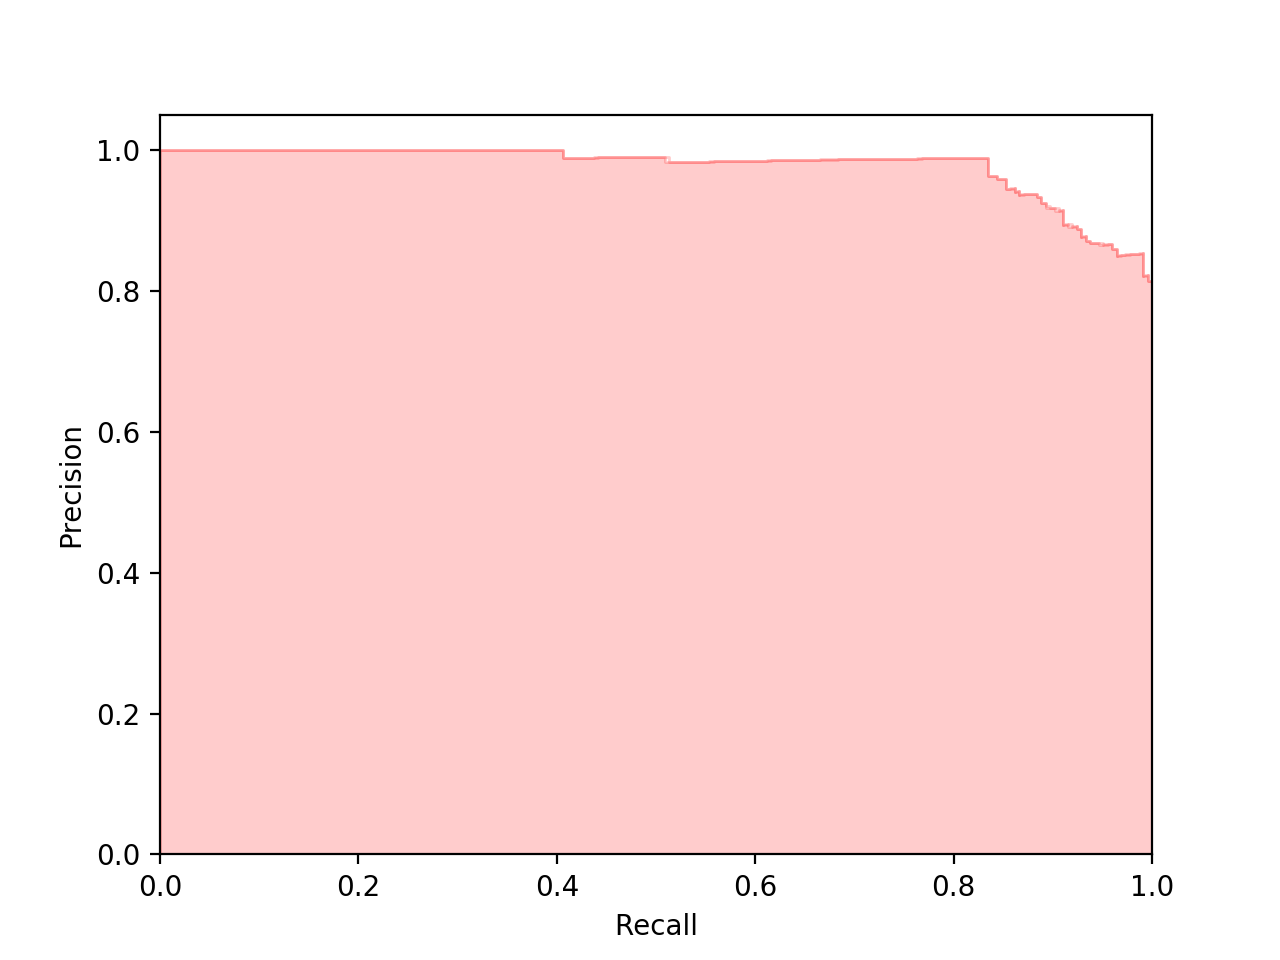
\includegraphics[width=\textwidth]{graphics/nns/cnn}
		\caption{Architecture of the Convolutional Neural Network}
		\label{Fig: impl/ml/cnn/architecture}
	\end{figure}
	The first layer performs batch normalization on the input data and then passes it to the first convolutional layer. Each of the three convolutional layers uses a separate $1\times2$ kernel, which is learned during training. Figure \ref{Fig: impl/ml/cnn/compGraph} shows the computational graph of the first two convolutional layers, while Figure \ref{Fig: impl/ml/cnn/compGraphLast} shows the computational graph for the last convolutional layer, which also performs dropout regularization with keep probability $k_p = 0.8$.
	\begin{figure}[H]
		\centering
		\begin{subfigure}[b]{.4\textwidth}
			\centering
			\includegraphics[width=.7\textwidth]{graphics/nns/cnn-compGraph}
			\caption{First two convolutional layers}
			\label{Fig: impl/ml/cnn/compGraph}
		\end{subfigure}
		\hfill
		\begin{subfigure}[b]{.4\textwidth}
			\centering
			\includegraphics[width=.7\textwidth]{graphics/nns/cnn-compGraphLast}
			\caption{Last convolutional layer}
			\label{Fig: impl/ml/cnn/compGraphLast}
		\end{subfigure}
		\caption{Computational graphs for the convolutional layers.}
		\label{Fig: impl/ml/cnn/compGraphs}
	\end{figure}
	The activation functions of the dense and output layers are ReLU and softmax, respectively. Figure \ref{Fig: impl/ml/mlp/compgraph} pictures the computational graphs for these two layers. 
	\\ \\
	Just like the MLP, the CNN optimizes the parameters using the Adam algorithm and the \textbf{binary crossentropy} loss function with weight decay regularization (Equation \ref{Eq: impl/ml/loss}).
 
	\subsection{Probabilistic Neural Network} \label{Section: impl/ml/pnn}
	The implementation of the Probabilistic Neural Network (PNN) consisted of two major algorithms: training and classification.
	\subsubsection*{PNN training}
	The first step in training the PNN is normalizing each pattern vector $\mathbf{x}$ to have unit length (i.e. $\vert\vert \mathbf{x}\vert\vert = 1$). Each normalized training pattern is then placed on the input units and the weights linking them to the pattern units are set such that $\mathbf{w}_i = \mathbf{x}_i$. Then, a single connection from the pattern unit is made to the category unit corresponding to the class of the input pattern. Algorithm \ref{Alg: impl/ml/pnn/train} outlines the pseudocode of this algorithm.
	\begin{algorithm}[H]
		\caption{PNN training algorithm}
		\label{Alg: impl/ml/pnn/train}
		\begin{algorithmic}
			\Procedure{train\_PNN}{}
				\State $j \gets 0$
				\State $n \gets \text{number of patterns}$ 
				\Do
					\State $j \gets j + 1$
					\State $x_{jk} \gets \frac{x_{jk}}{\sqrt{\sum_{i=1}^{d}x_{ij}^2}}$ \Comment{\textbf{normalization}}
					\State $w_{jk} \gets x_{jk}$ \Comment{\textbf{setting weight values}}
					\If{$\mathbf{x} \in \omega_i$}
						\State $a_ic \gets 1$
					\EndIf
				\doWhile{$j \neq n$}
			\EndProcedure
		\end{algorithmic}
	\end{algorithm}
	After the training phase, the PNN will be fully connected between input and pattern units and sparsely connected from pattern to category units. Figure \ref{Fig: impl/ml/pnn/architecture} shows the architecture of the PNN resulting from this algorithm.
	\begin{figure}[H]
		\centering
		\includegraphics[width=.8\textwidth]{graphics/nns/pnn-impl}
		\caption{PNN architecture}
		\label{Fig: impl/ml/pnn/architecture}
	\end{figure}
	\subsubsection*{PNN classification}
	When we want to classify a new pattern, $\mathbf{x}$, we first normalize it and then place it at the input units. Each pattern unit then computes the inner product:
	\begin{equation}
		z_k = \mathbf{w}_k^T \mathbf{x}
		\label{Eq: impl/ml/pnn/innerprod}
	\end{equation}   
	and emits $\exp(\frac{z_k-1}{\lambda^2})$, where $\lambda$ is a parameter set to be $\sqrt{2}$ times the width of the effective Gaussian window. The reasoning behind this nonlinearity is outlined in the Appendix \ref{Appendix: Parzen/math-background}, Section \ref{Section: appendix/pnn/parameter}.
	\\ \\
	Each category unit then sums the outputs of the pattern units connected to it. Thus, each pattern unit contributes to its associated category unit with a signal equal to the probability that the test pattern $\mathbf{x}$ was generated by a Gaussian centred on the associated training point. The sum of these local estimates gives $g_i(\mathbf{x})$ - the Parzen window estimate of the underlying distribution. The resulting class is then given by $\argmax_i g_i(\mathbf{x})$ (Algorithm \ref{Alg: impl/ml/pnn/classify}). 
	\begin{algorithm}[H]
	\caption{PNN classification algorithm}
	\label{Alg: impl/ml/pnn/classify}
	\begin{algorithmic}[H]
		\Procedure{classify\_PNN}{$\mathbf{x}$}
		\State $\mathbf{x} = \text{normalize}(\mathbf{x})$
		\State $k \gets 0$
		\State $n \gets \text{number of patterns}$ 
			\Do
				\State $k \gets k + 1$
				\State $z_k \gets \mathbf{w_k}^T\mathbf{x}$
				\If{$a_{kc} = 1$}
					\State $g_c \gets g_c + \exp(\frac{z_k - 1}{\sigma^2})$
				\EndIf
			\doWhile{$k \neq n$} 
		\State $class \gets \argmax_i g_i(\mathbf{x})$ \\
		\Return{class}
		\EndProcedure
	\end{algorithmic}
	\end{algorithm}
	The training algorithm only requires one pass through the training data and therefore the PNN is significantly faster at learning than the parametric methods, such as the MLP. The space complexity can be easily determined by counting the number of wires in Figure \ref{Fig: impl/ml/pnn/architecture}: $O((n+1)d)$, where $n$ is the number of patterns in the training set and $d$ is the length for each pattern. The time complexity for classification is $O(n)$, but can be done in $O(1)$ by computing the inner products from equation \ref{Eq: impl/ml/pnn/innerprod} in parallel. Therefore, the PNN is highly applicable to my problem, as I don't have limited storage availability and classification speed is a key requirement for the API. 
	
	\section{REST API} \label{Section: impl/REST}
	This section describes how the REST API module was implemented.
	\subsection{Requests handling} \label{Section: impl/REST/actual}
	The main entry point to the REST API receives a POST HTTP request from the client, containing a JSON file with a list of nodes to classify. Each node in the list will be represented by a (\textit{uuid}, \textit{timestamp}) pair, which allows the tool to uniquely identify it in the Neo4J database. The API then initiates a 'job' that starts classifying the nodes in background and replies with a JSON containing its ID.
	\\ \\
	Using this job ID, the client can then query the API using an HTTP GET request and the API will reply with a different JSON containing the list of nodes that have been classified so far and the status of the job, which can be one of: \textit{WAITING} (meaning that it is idle), \textit{RUNNING}(representing that the job is still classifying nodes and therefore the results returned are partial) and \textit{DONE} (meaning that the job is finished and the classification results are for the entire set of nodes queried initially). 
	\\ \\
	I decided to implement this two-step mechanism considering that node classification takes a long time, especially when working with large databases. This way, the client sends a request and can then query the API at any time for the job status and partial or final classification results. 
	\\ \\
	Another key factor that I took into consideration is how the API will treat different types of nodes, considering that the machine learning models only apply to \textit{File}, \textit{Socket} and \textit{Process} nodes. Table \ref{Table: impl/REST/API-strategy} shows the strategies adopted by the API for different types of nodes.
	\begin{longtable}{|p{.15\textwidth}|p{.85\textwidth}|}
		\textbf{Node type} & \textbf{API strategy} \\
		\hline
		\textit{File} & \multirow{3}{*}{Return the classification result for the node.} \\
		\textit{Socket} & \\
		\textit{Process} & \\
		\hline
		\textit{Machine} & Only $0.00178\%$ of the total number of nodes, so consider classified as \textit{SHOW} by default. \\
		\hline
		\textit{Meta} & \multirow{2}{*}{Return the classification result for the \textit{Process} node that it is connected to.} \\
		\textit{Pipe} & \\
		\hline
		\caption{API strategy for different type of nodes.}
		\label{Table: impl/REST/API-strategy}
 	\end{longtable}
 
	\subsection{Caching mechanism} \label{Section: impl/REST/caching}
	Due to the stateless nature of REST APIs, caching is a desirable feature in order to avoid a high load on the application. Moreover, an efficient caching mechanism is essential to support the 2-step format of the API described previously. 
	\\ \\
	In order to handle caching, I am using a PostgreSQL database. PostgreSQL is an open source and highly customizable SQL dialect, providing stored procedures in more than a dozen programming languages, including Java, Perl and Python. 
	\\ \\
	The actual database structure is made of three tables: \textit{Jobs} (storing all the jobs processed by the server and their status), \textit{Nodes} (storing the cached results for the nodes) and \textit{JobsToNodes} (storing the relationships between jobs and nodes). The full relational schema is shown in Figure \ref{Fig: impl/REST/cache/relational}.
	\begin{figure}[H]
		\centering
		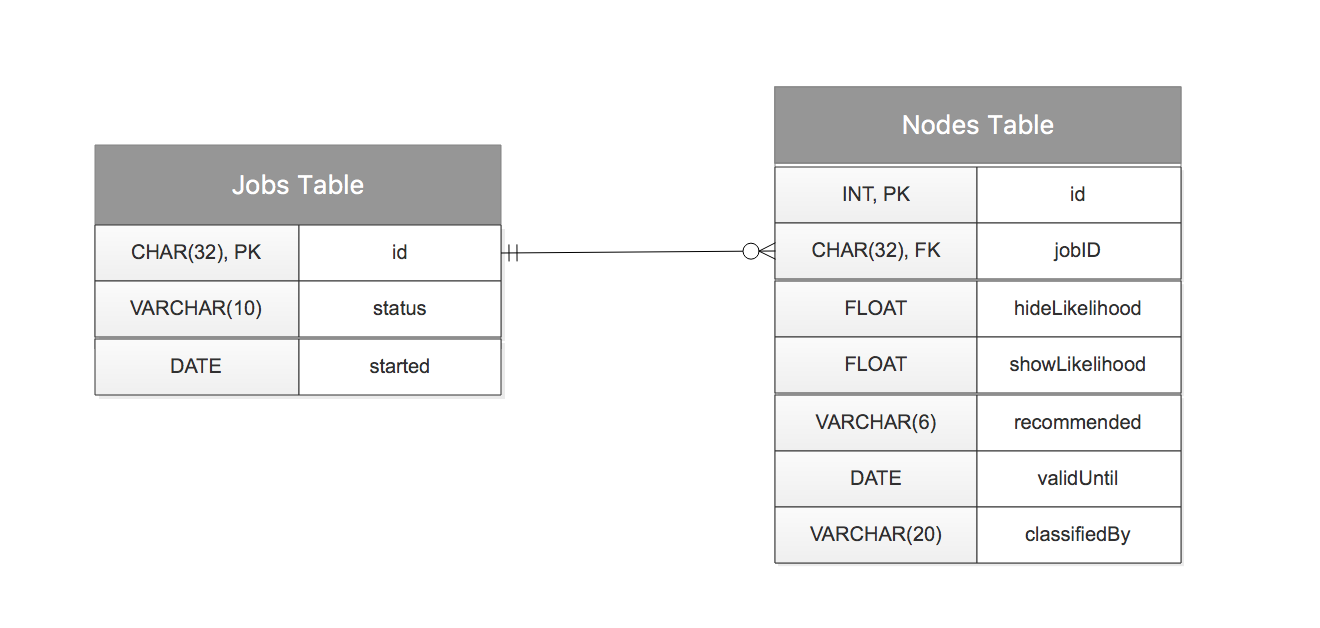
\includegraphics[width=\textwidth]{graphics/cache-schema}
		\caption[Cache schema]{Relational schema used by the caching mechanism.}
		\label{Fig: impl/REST/cache/relational}
	\end{figure}
	By default, every cache entry is invalidated 72 hours after the job that the node is associated with is finished. On top of this, the API provides an entry point for forcibly clearing the cache. 
	\\ \\
	Figure \ref{Fig: impl/REST/cache/jobs} shows the UML diagram of the core classes of the REST API.
	\begin{figure}[H]
		\centering
		\includegraphics[width=.9\textwidth]{graphics/umls/jobs-uml}
		\caption{UML diagram of server-side job handling.}
		\label{Fig: impl/REST/cache/jobs}
	\end{figure}
	
	\section{Software engineering practices} \label{Section: impl/SoftEngPractices}
	In this section I will present the software engineering practices that were followed throughout the implementation stage. These practices where essential, especially considering the fact that the project has a codebase of almost $3,000$ lines of code\footnote{Calculated using the open-source tool \textbf{cloc}: \textbf{\url{https://github.com/AlDanial/cloc}}}. 
	\\ \\
	Firstly, I divided the project into three core modules that interact with one another and can easily be tested and optimised separately. In order to achieve this, every module makes use of the object-oriented paradigm. Moreover, this allows anyone who wants to extend the tool to do so with ease, by simply extending one class and specifying this when starting the API.  
	\\ \\
	The connection between the three modules only depends on three classes: \textit{RequestJob}, \textit{Model} and \textit{DatabaseDriver} (Figure \ref{Fig: impl/REST/API-integrate}). This way, each module can be extended separately, without interfering with the other two, guaranteeing their independence.  
	\begin{figure}[H]
		\centering
		\includegraphics[width=.9\textwidth]{graphics/umls/uml-connections}
		\caption[General UML diagram]{\centering UML diagram showing the integration of the three modules.}
		\label{Fig: impl/REST/API-integrate}
	\end{figure}
	Another goal I set was the scalability of the API. For this reason, I decided to use a REST-like architecture, which allows this module to scale horizontally, by balancing the load between multiple instances of the server. The cache can then be either shared by all the instances, or have one cache for each instance. In both cases, though, the cache database can be scaled vertically by running it on a more powerful machine. 
	\\ \\
	I also made use of the new features provided by Python $3.6$ by \textit{statically typing} the functions' arguments and return types. In order to ensure their correct behaviour, I wrote unit tests for most of the core functionalities of the project.
	\section{Summary} \label{Section: impl/summary}
	In this chapter I described the implementation of the three core modules of the project and their interaction. For every module, I described the limitations and difficulties I encountered and I motivated the decisions took when designing them. 
	\\ \\
	The following chapter will first show the results of evaluating the tool from multiple points of view(such as model performance or server service time) and then discuss these results. Furthermore, the next chapter also includes a comparative evaluation of the models from which I can decide which would be more appropriate in practice. 
\end{document}